%----------------------------------------------------------------------
%	REQUIRED PACKAGES
%----------------------------------------------------------------------
\documentclass[12pt]{report}
\usepackage[numbers,sort&compress]{natbib}
\usepackage[utf8]{inputenc}
\usepackage{amsmath,amsfonts,amssymb}
\usepackage{graphicx}
\usepackage{tikz}
\usepackage{float}
\usepackage{placeins}
\usepackage{url}
\usepackage{caption}
\usepackage{setspace}
\usepackage{tocloft}

%----------------------------------------------------------------------
%	FONTS,INDENTATION, MARGINS, LINE SPACING
%----------------------------------------------------------------------
\usepackage{times}      % Loads the Times-Roman Fonts
\usepackage{mathptmx}   % Loads the Times-Roman Math Fonts
\usepackage[left=3.81cm,
            right=2.54cm,
		top=2.54cm,
		bottom=2.54cm,
		a4paper]{geometry}
  
\setlength{\parindent}{0pt} % Remove paragraph indent globally
\usepackage{setspace} %package for line spacing
\setstretch{1.5}
\usepackage{parskip}
\setlength{\parskip}{6pt}  % Adjust paragraph spacing as needed

%----------------------------------------------------------------------
%	TITLES,SECTIONS,SUBSECTIONS AND SUBSUBSECTIONS
%----------------------------------------------------------------------
\usepackage{titlesec}
\titlespacing{\chapter}{0pt}{-24pt}{12pt}
\titlespacing{\section}{0pt}{16pt}{16pt}
\titlespacing{\subsection}{0pt}{16pt}{16pt}
\titlespacing{\subsubsection}{0pt}{16pt}{16pt}

\titleformat{\chapter}[display]{\centering\fontsize{14pt}{12pt}\bfseries}{\MakeUppercase{\chaptertitlename\ \thechapter}}{12pt}{}
\titleformat{\section}{\fontsize{12pt}{16pt}\bfseries\raggedright}{\thesection}{0.5em}{}
\titleformat{\subsection}{\fontsize{12pt}{16pt}\bfseries\raggedright}{\thesubsection}{0.5em}{}
\titleformat{\subsubsection}{\fontsize{12pt}{16pt}\bfseries\raggedright}{\thesubsubsection}{0.5em}{}
\titleformat{\paragraph}{\fontsize{12pt}{0pt}\bfseries\raggedright}{\theparagraph}{0.5em}{}

%----------------------------------------------------------------------
%	FORMATTING THE TABLE OF CONTENTS,LOF AND LOT
%----------------------------------------------------------------------

% Adjust the spacing for the TABLE OF CONTENT
\renewcommand{\cftbeforetoctitleskip}{-18pt} % Space before the TOC title
\renewcommand{\cftaftertoctitleskip}{12pt} % Space after the TOC title
\renewcommand{\cftbeforechapskip}{9pt} % Space before each chapter entry
\renewcommand{\cftbeforesecskip}{9pt} % Space before each section entry
\renewcommand{\cftbeforesubsecskip}{9pt} % Space before each section entry
\renewcommand{\contentsname}{\fontsize{14}{16}\bfseries TABLE OF CONTENTS}

% Adjust the spacing for the LIST OF FIGURES
\renewcommand{\cftbeforeloftitleskip}{-18pt} % Space before the LOF title
\renewcommand{\cftafterloftitleskip}{12pt} % Space after the LOF title
\renewcommand{\cftbeforefigskip}{10pt} % Space before each figure entry
\renewcommand{\listfigurename}{\fontsize{14}{16}\bfseries LIST OF FIGURES}
\renewcommand{\cftfigpresnum}{\figurename\ }
\renewcommand{\cftfigaftersnum}{:}
\renewcommand{\cftfigaftersnumb}{\hspace{2.5em}} 

% Adjust the spacing for the LIST OF TABLES
\renewcommand{\cftbeforelottitleskip}{-18pt} % Space before the LOT title
\renewcommand{\cftafterlottitleskip}{12pt} % Space after the LOT title
\renewcommand{\cftbeforetabskip}{10pt} % Space before each table entry
\renewcommand{\listtablename}{\fontsize{14}{16}\bfseries LIST OF TABLES}
\renewcommand{\cfttabpresnum}{Table\ }
\renewcommand{\cfttabaftersnum}{:}
\renewcommand{\cfttabaftersnumb}{\hspace{2.5em}}

%----------------------------------------------------------------------
%	END OF PREAMLBE AND BEGINNING OF THE DOCUMENT
%----------------------------------------------------------------------

\begin{document}

\pagenumbering{roman} % roman page numbers
\begin{titlepage}
    \centering
    
    
\includegraphics[width=0.2\textwidth]{Graphics/TULogo.png}\par
    \vspace{1.2cm}
    {\fontsize{14pt}{12pt}\selectfont\bfseries\textcolor{black}
    TRIBHUVAN UNIVERSITY \par INSTITUTE OF ENGINEERING \par PURWANCHAL CAMPUS \par
    \vspace{1.2cm}
    \begin{flushleft}
    
    \end{flushleft}

\begin{center}
    A MINOR PROJECT REPORT ON \\
    A DECENTRALIZED SOCIAL MEDIA FOR SCIENTIFIC COMMUNICATION
\end{center}

    \vspace{1.2cm}
    BY\par Rijan Karki(PUR078BCT067)
      \par Saurav Khanal(PUR078BCT080)
      \par Spandan Guragain(PUR078BCT086)
      \par Sudesh Subedi(PUR078BCT088)
    \vspace{1.2cm}\par
    }
    {\fontsize{13pt}{12pt}\selectfont\bfseries\textcolor{black}
    DEPARTMENT OF ELECTRONICS AND COMPUTER ENGINEERING\par PURWANCHAL CAMPUS\par DHARAN, NEPAL\par
    \vspace{1.2cm}
    \vspace{1.2cm}
    
    FEBRUARY,2025 
    }
\end{titlepage}

\chapter*{ACKNOWLEDGEMENT}
\addcontentsline{toc}{chapter}{ACKNOWLEDGEMENT}

We would like to express our sincere gratitude to our supervisor Mr. Pukar Karki, Deputy Head of the Department, for his invaluable guidance and unwavering support throughout the preparation of this report. Their insightful suggestions and constructive feedback have been instrumental in shaping our work, and we are truly appreciative of the time and effort they dedicated to our development. Their leadership has not only provided us with direction but has also inspired us to pursue excellence in our academic endeavors.

We are also deeply thankful to our esteemed teachers and faculty members for their encouragement and thoughtful insights, which have significantly enriched this proposal. Their commitment to academic excellence and their willingness to share knowledge have served as a constant source of inspiration for us. The collective guidance and support we received from them have greatly contributed to the refinement and improvement of our work, and we are sincerely grateful for their contributions.

\vspace{1cm}
\textbf{Rijan Karki} 
PUR078BCT067\\
\textbf{Saurav Khanal} 
PUR078BCT080\\
\textbf{Spandan Guragain} 
PUR078BCT086\\
\textbf{Sudesh Subedi} 
PUR078BCT088\\

\chapter*{ABSTRACT}
\addcontentsline{toc}{chapter}{ABSTRACT}

Abstract goes here.

{\centering{\tableofcontents}}\newpage
{\centering\listoffigures\addcontentsline{toc}{chapter}{LIST OF FIGURES}}
\newpage
\newpage
\chapter*{LIST OF ABBREVIATIONS}
% \vspace{1cm}
\addcontentsline{toc}{chapter}{LIST OF ABBREVIATIONS}
\begin{tabular}{l l}
API	&	:	Application Programming Interface	\\
UI	&	:	User Interface \\
W3C	&	:	World Wide Web Consortium \\


\end{tabular}









\pagenumbering{arabic}
\chapter{INTRODUCTION}
\section{Background}
Scientific communication plays a vital role in advancing research and knowledge sharing across academic communities. Traditional social media platforms while effective for general communication often lack specialized features necessary for scientific discource. The emergence of decentralized technologies particularly the ActivityPub \cite{ActivityPub} Protocol and the Fediverse presents an oppurtunity to create a more suitable platform for academic communication. 
\section{Gap Identification}
Current platforms for scientific communication face several limitations:

\begin{itemize}
  \item Limited accessibility of scientific communication to the broader population beyond niche communities.
  \item Insufficient support for mathematical expressions and scientific notations.
  \item Lack of integration with academic citation systems.
  \item Reliance on a third party for the protection and moderation of user data.
\end{itemize}

\section{Motivation}
To create a social media platform that empowers researchers and academics to communicate their scientific work effectively. By bridging the gap between specialized communities and the general public, the platform aims to promote the understanding and appreciation of cutting-edge research across a wider audience. Along with the ability to run individual servers by individual people/institutions without losing the ability to communicate between each other.

\section{Objectives}
\begin{itemize}
  \item Develop a federated social media platform using the ActivityPub protocol with support for mathematical and scientific typesetting.
  \item Streamline the server setup process to enable technically literate individuals to host their own servers with minimal effort.
\end{itemize}

\chapter{RELATED THEORY}

\section{Decentralization}
Decentralization refers to the distribution of authority, control, and decision-making away from a central authority. In the context of digital platforms, decentralization allows users to maintain control over their data and interactions, fostering a more democratic and resilient online environment. This approach contrasts with traditional centralized systems, where a single entity governs all operations and data management. 
\begin{figure}[h]
  \centering
    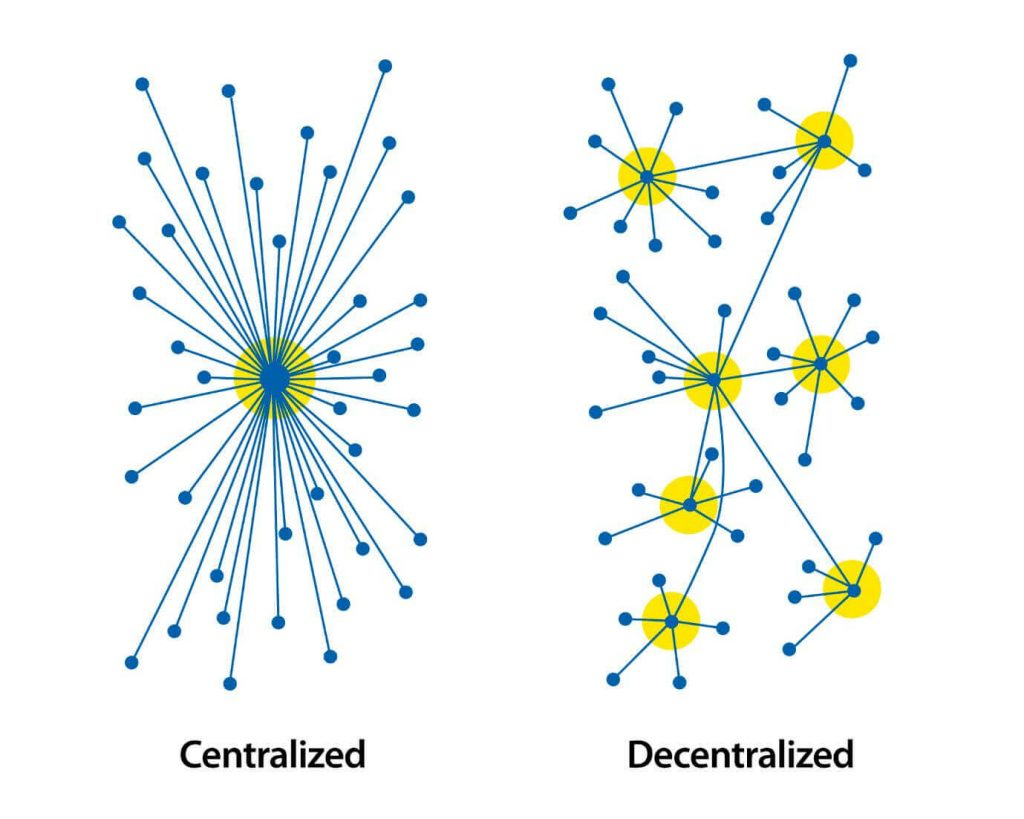
\includegraphics[width=0.75\textwidth]{Graphics/centvsdecent.jpg} % Adjust the width as needed
    \caption{The structure of a centralized network compared to a decentralized network.}
    \label{fig:example}
\end{figure}
\section{Federation}
Federation is a model that enables different systems or organizations to interoperate while maintaining their independence. In social media, a federated approach allows users from different platforms to communicate and share content seamlessly, creating a more interconnected online community. This is achieved through protocols that facilitate data exchange and interaction across diverse platforms.

\section{Scientific Typesetting}
Scientific typesetting involves the formatting of mathematical and scientific content for clarity and precision. It is essential for effectively communicating complex ideas in academic and research contexts. Proper typesetting ensures that equations, symbols, and notations are presented in a way that is easily understandable and visually appealing. The prime example of a Scientific Typesetting is LaTeX but there are alternatives like AsciiMath and Typst.

\section{ActivityPub Protocol}
ActivityPub is a decentralized social networking protocol standardized by the World Wide Web Consortium (W3C) \cite{ActivityPub}. It provides a client-to-server API for creating, updating, and deleting content, as well as a server-to-server API for delivering notifications and content between different servers. 

The federation model offers several key advantages over centralized systems, such as resilience (no single point of failure as the network operates across multiple independent servers), data sovereignty (each instance maintains control over its users' data and policies), interoperability (users can communicate across instances using standardized protocols), and scalability (the network can grow organically as new instances join the federation).
\begin{figure}[h]
  \centering
    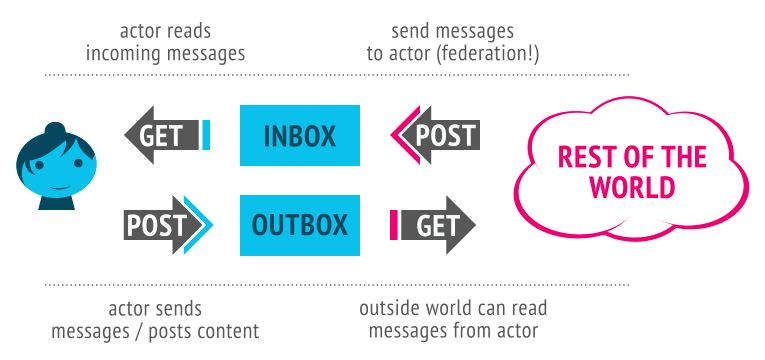
\includegraphics[width=0.95\textwidth]{Graphics/activitypubexample.png} % Adjust the width as needed
    \caption{Communication using ActivityPub Protocol.}
    \label{fig:example}
\end{figure}

 The protocol is built on several key concepts:

\begin{itemize}
  \item \textbf{Actors} which represent users, groups, or applications that can send and receive activities.
  \item \textbf{Activities} which describe actions that actors take.
  \item \textbf{Objects} which represent the content being acted upon.
\end{itemize}


\chapter{LITERATURE REVIEW}

\section{Related Works}

The Fediverse connects various decentralized social networks, allowing users to interact across different platforms. This section reviews some of the prominent projects within the Fediverse.

\begin{itemize}
  \item \textbf{Mastodon}\cite{mastodon}\\
    Mastodon is a decentralized social network that operates on open-source software. It allows users to create their own servers (instances) and interact with users on other instances. Mastodon emphasizes user privacy and control over content, providing features like content warnings and robust moderation tools.

  \item \textbf{Pixelfed}\cite{pixelfed}\\
    Pixelfed is a federated image-sharing platform similar to Instagram. It focuses on user privacy and data ownership, allowing users to share photos and interact with others without centralized control. Pixelfed supports ActivityPub, enabling interaction with other Fediverse platforms.

  \item \textbf{PeerTube}\cite{peertube}\\
    PeerTube is a decentralized video hosting platform that uses peer-to-peer technology to distribute video content. It aims to provide an alternative to centralized video platforms like YouTube, giving users control over their content and reducing reliance on centralized servers. PeerTube instances can federate with each other, allowing for a distributed network of video content.

  \item \textbf{Lemmy}\cite{lemmy}\\
    Lemmy is a federated link aggregation and discussion platform similar to Reddit. It allows users to create and join communities, share links, and engage in discussions. Lemmy instances can federate with each other, enabling a decentralized network of communities.

\end{itemize}

\section{Decentralization and Federation}

Decentralization and federation are key concepts in the Fediverse. Decentralization refers to the distribution of data and control across multiple servers, reducing reliance on a single central authority. Federation allows different servers to communicate and interact with each other, creating a network of interconnected platforms.

\subsection{Benefits of Decentralization}

Decentralization offers several benefits, including:

\begin{itemize}
  \item \textbf{Privacy and Control}: Users have greater control over their data and privacy settings, as there is no central authority collecting and monetizing user data.
  \item \textbf{Resilience}: Decentralized networks are more resilient to censorship and outages, as there is no single point of failure.
  \item \textbf{Community Governance}: Users can create and govern their own instances, fostering diverse and self-sustaining communities.
\end{itemize}

\subsection{Challenges of Decentralization}

Despite its benefits, decentralization also presents challenges:

\begin{itemize}
  \item \textbf{Interoperability}: Ensuring seamless interaction between different platforms and instances can be complex.
  \item \textbf{Moderation}: Decentralized networks require robust moderation tools to manage content and prevent abuse.
  \item \textbf{Scalability}: Decentralized systems must be designed to handle large numbers of users and high volumes of data.
\end{itemize}

\section{Protocols and Technologies}

The Fediverse relies on various protocols and technologies to enable decentralization and federation. Some of the key protocols include:\\

\begin{itemize}
  \item \textbf{ActivityPub}\cite{ActivityPub}\\
    ActivityPub is a decentralized social networking protocol used by many Fediverse platforms. It enables users to follow, share, and interact with content across different instances.

  \item \textbf{WebFinger}\cite{webfinger}\\
    WebFinger is a protocol for discovering information about people and resources on the internet. It is used in the Fediverse to locate user profiles and instances.
\end{itemize}

\section{Conclusion}

The Fediverse represents a growing movement towards decentralized and federated social networks. By leveraging protocols like ActivityPub, platforms within the Fediverse offer users greater control over their data, enhanced privacy, and resilient communities. However, challenges such as interoperability, moderation, and scalability must be addressed to ensure the continued growth and success of decentralized social networks.


\chapter{METHODOLOGY}

Here we write about what metohods we used to make the project possible.

\chapter{IMPLEMENTAION}

Here we write about what we implementated and how.

\chapter{RESULTS}

\section{User \& Account Creation}

The platform follows a unique approach where each server is dedicated to a single user. However, within that server, the user can create and manage multiple accounts. This setup ensures full ownership and control over data while still enabling interaction within the federated network.

\subsection{User Creation}
To set up a user, the individual must provide a valid email address and set a secure password. This step ensures authentication and account recovery options. Once the user is registered, they gain full control over their server and can proceed to create multiple accounts as needed.

\begin{figure}[h!]
    \centering
    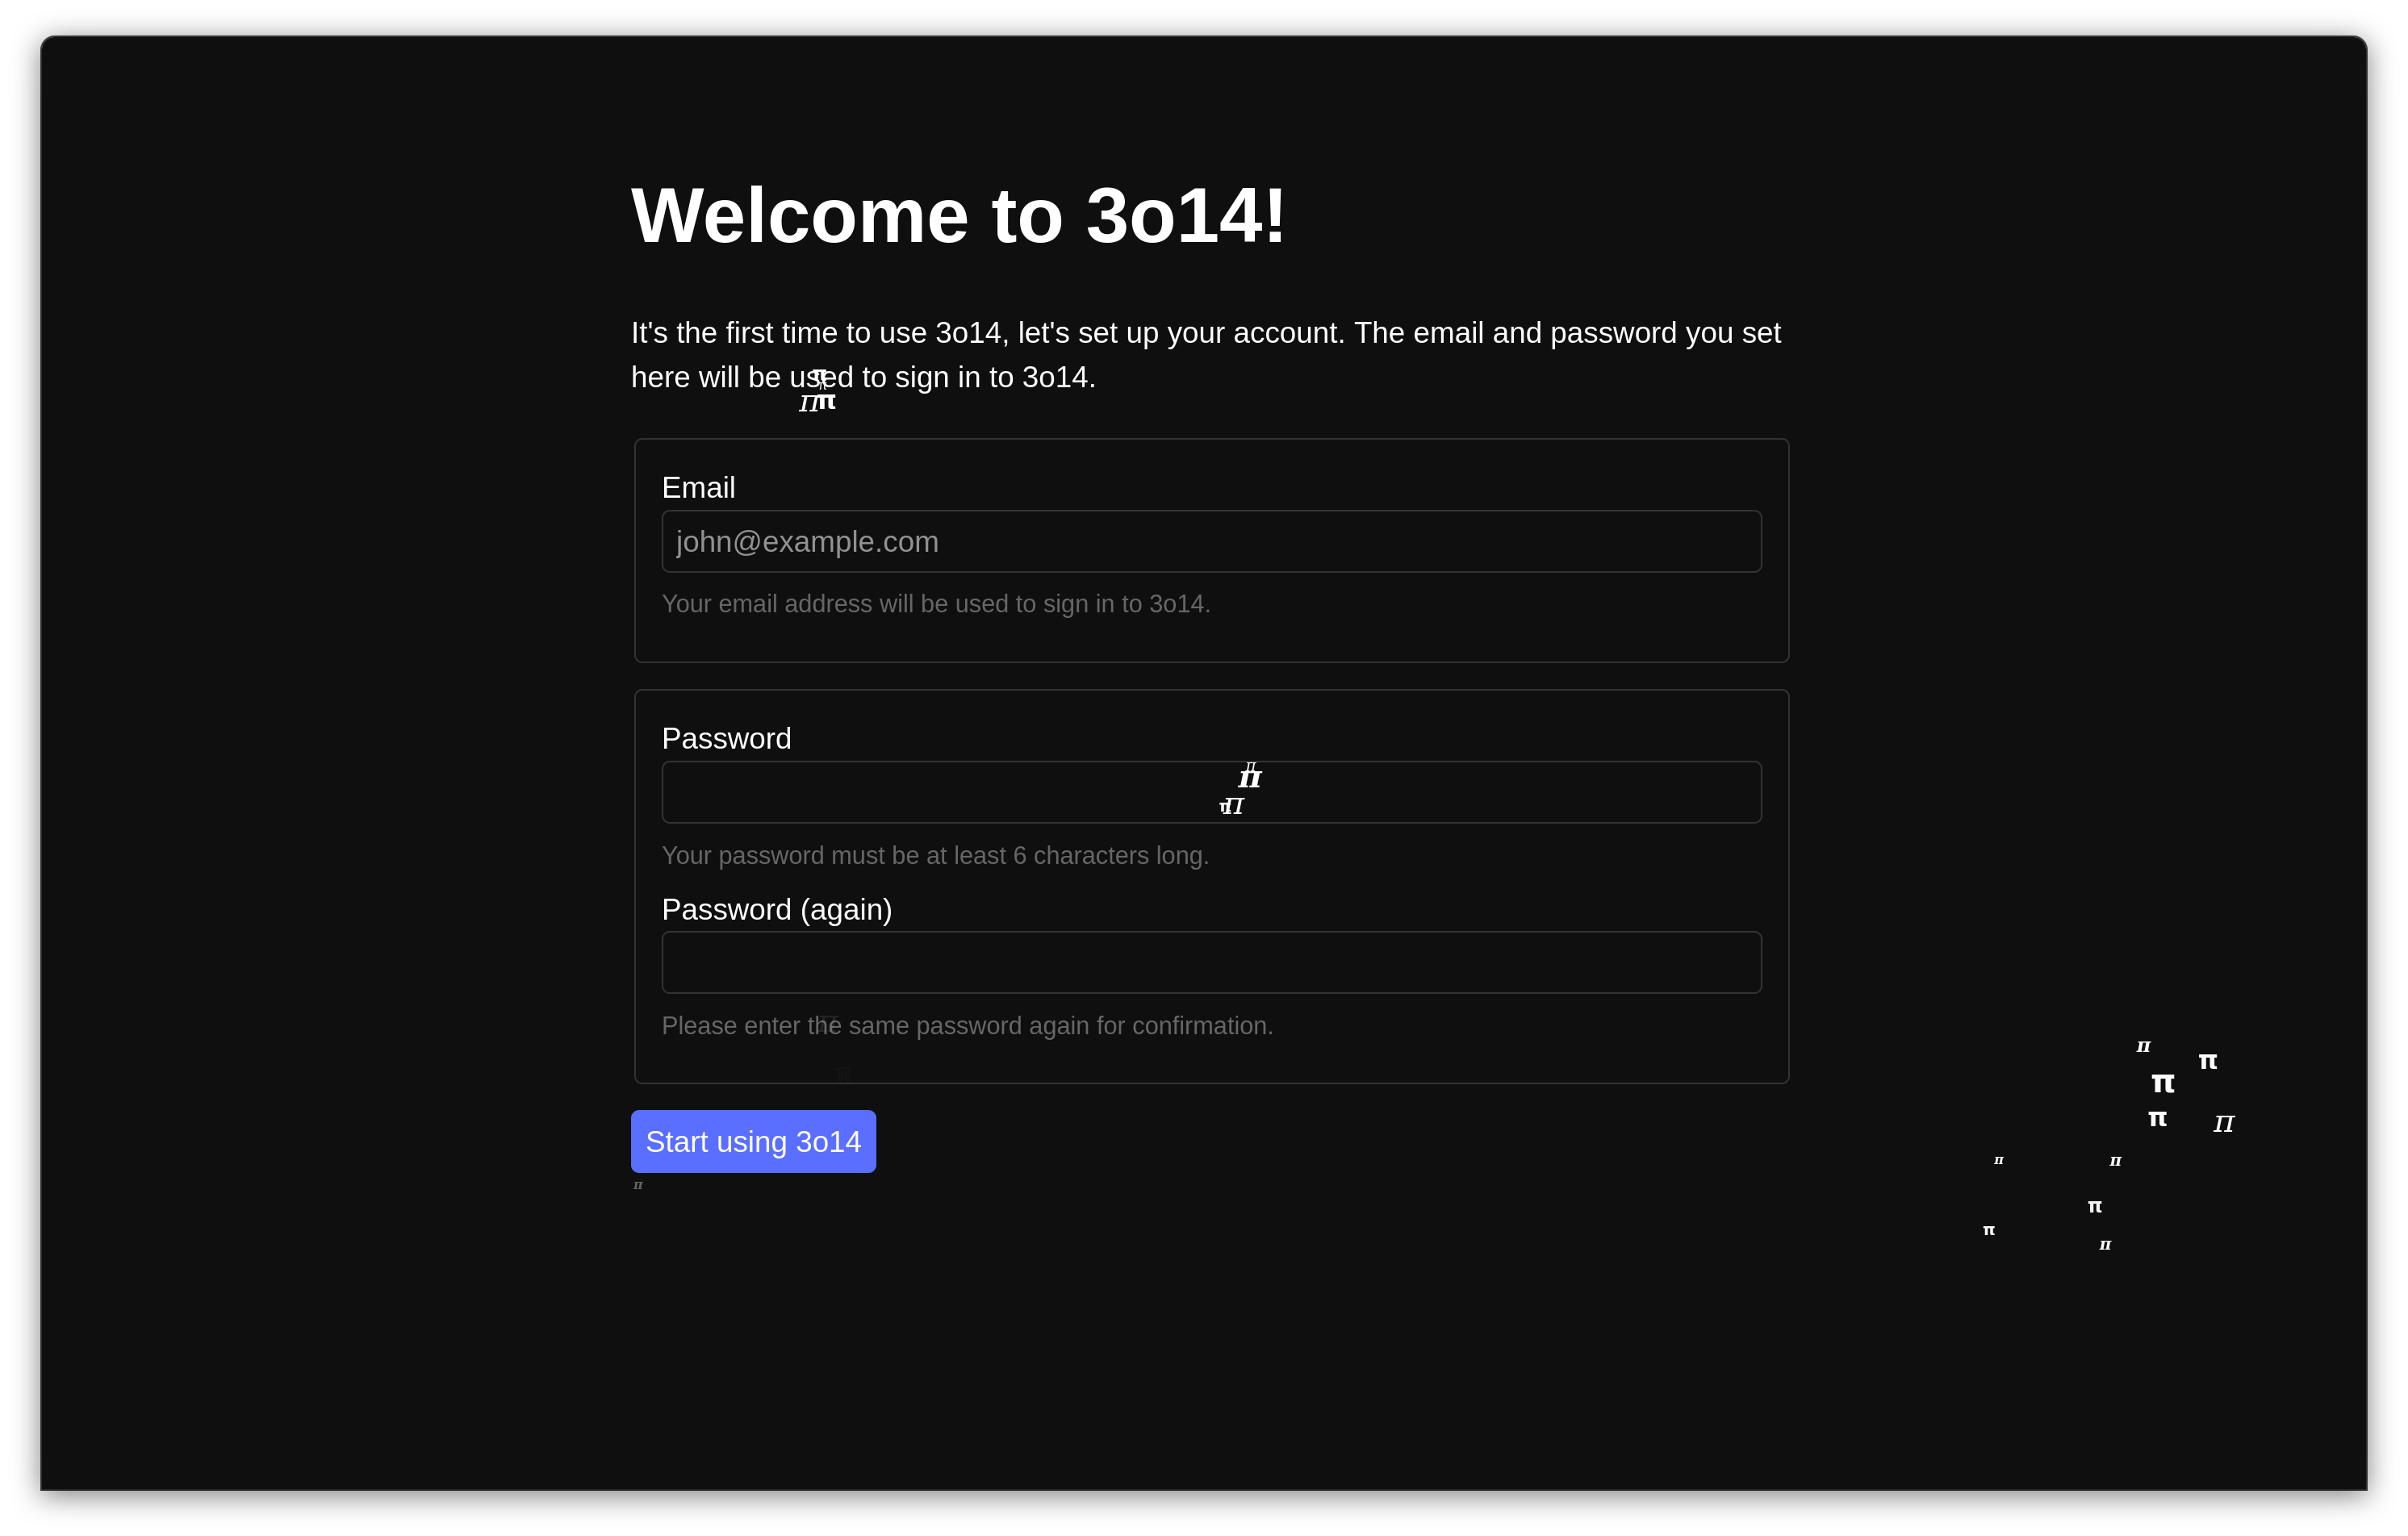
\includegraphics[width=0.5\textwidth]{Graphics/usercreation.png}
    \caption{User Creation}
    \label{fig:user_creation}
\end{figure}

\subsection{Account Creation}
Within their personal server, the user can create and manage multiple accounts. Each account can have distinct identities, preferences, and privacy settings while still operating under the same server. This feature allows for flexibility in communication, enabling users to maintain separate professional and personal identities, for example.

\begin{figure}[h!]
    \centering
    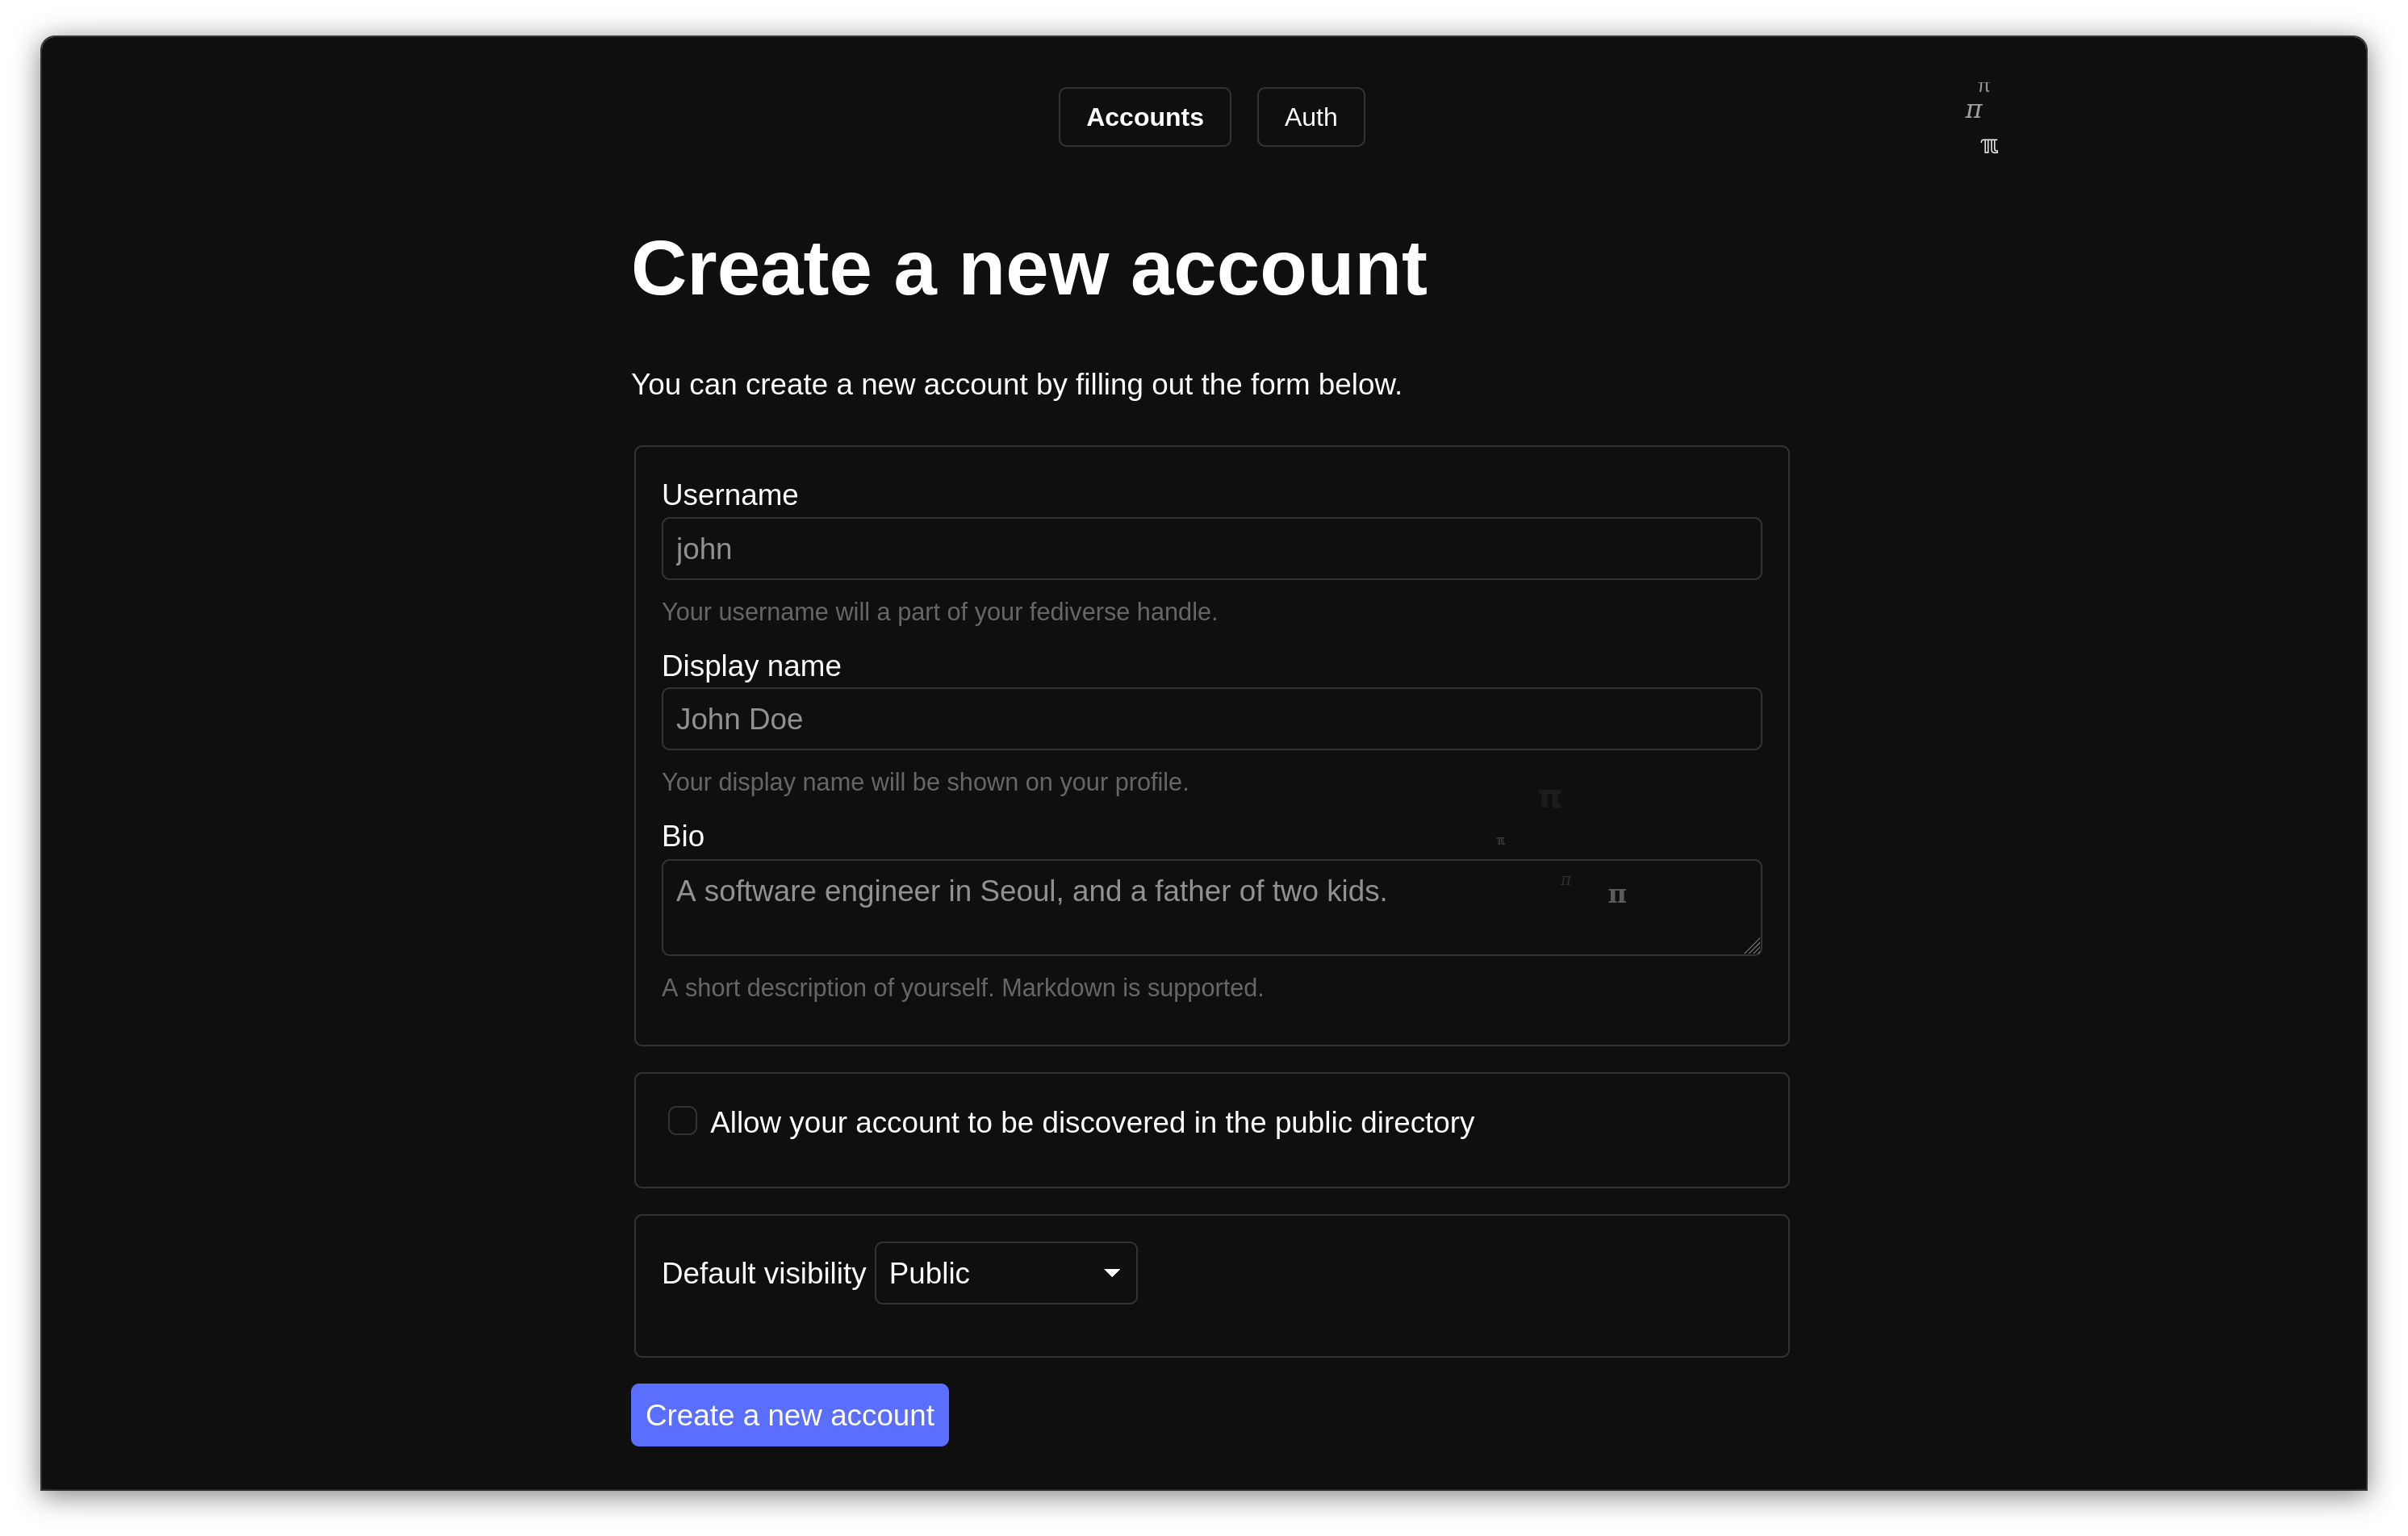
\includegraphics[width=0.5\textwidth]{Graphics/accountcreation.png}
    \caption{Account Creation}
    \label{fig:account_creation}
\end{figure}

\section{Posting Status With Latex}

Users can include mathematical expressions within plaintext using LaTeX syntax while composing a post. As shown in Figure~\ref{fig:writing_post}, the application provides a live preview of the rendered LaTeX output, allowing users to verify their equations before posting. Once published, the post is displayed in the timeline with properly formatted LaTeX expressions, as demonstrated in Figure~\ref{fig:post_in_timeline}. This feature ensures that complex mathematical notations, scientific formulas, and equations are easily readable and visually appealing in posts.

\begin{figure}[htbp]
  \centering
  % First image in its own minipage
  \begin{minipage}[b]{0.45\linewidth}
    \centering
    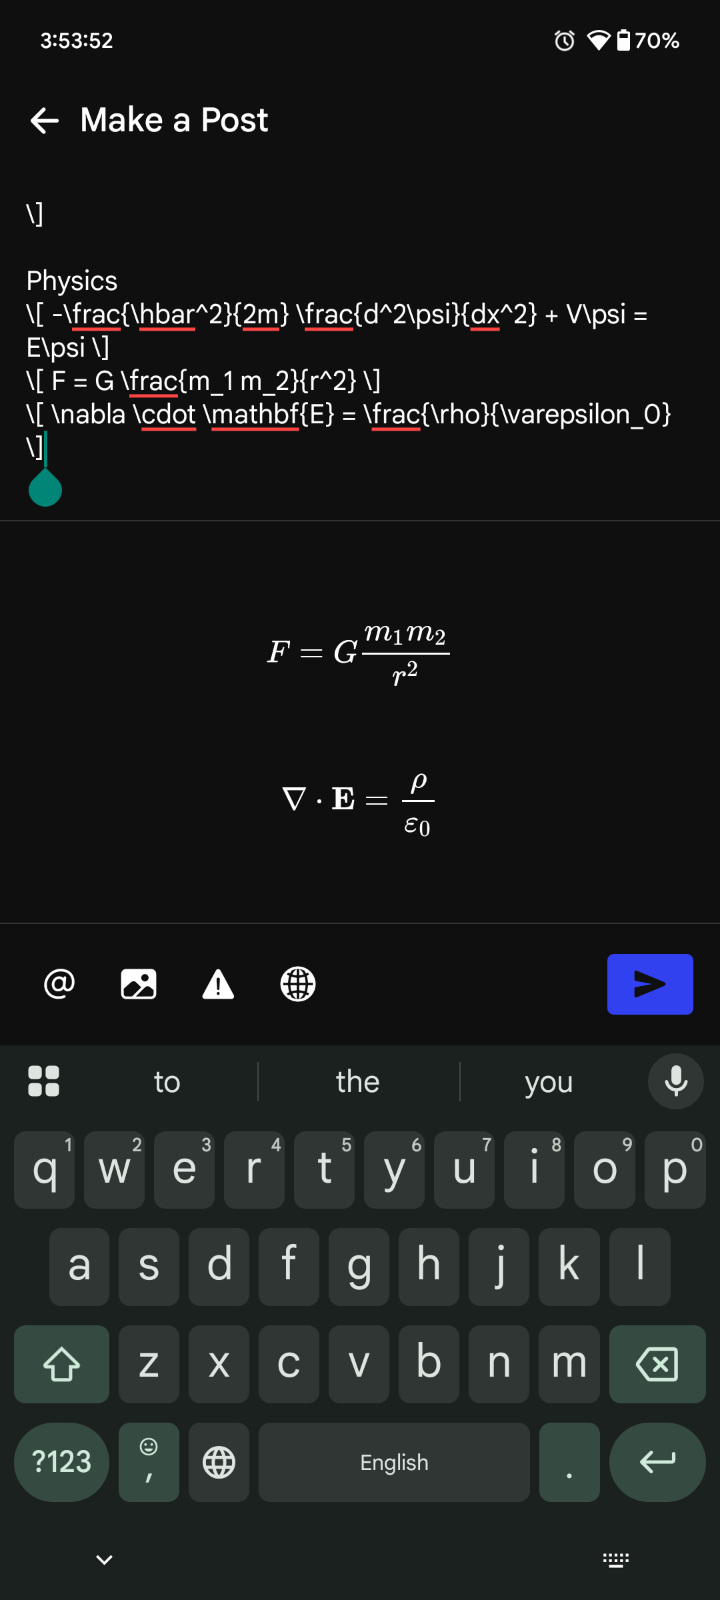
\includegraphics[width=\linewidth]{Graphics/writingpost.png}
    \caption{Live rendering of latex while writing post}
    \label{fig:writing_post}
  \end{minipage}
  \hfill % adds some space between images
  % Second image in its own minipage
  \begin{minipage}[b]{0.45\linewidth}
    \centering
    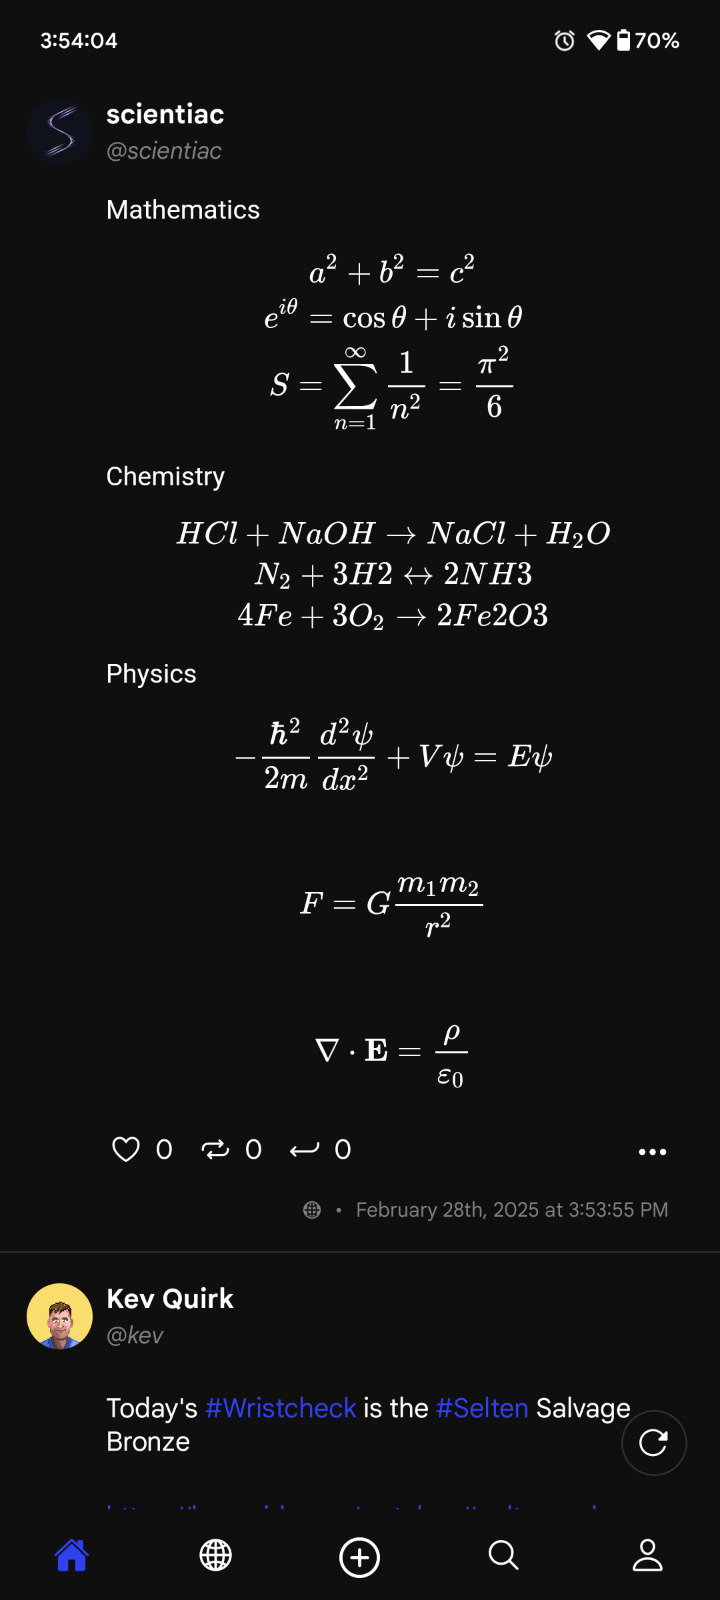
\includegraphics[width=\linewidth]{Graphics/postintimeline.png}
    \caption{Rendered post with latex in timeline}
    \label{fig:post_in_timeline}
  \end{minipage}
\end{figure}

\clearpage

\section{Interaction with Remote Accounts}
User, using their account, can interact with other users on different instances or services using ActivityPub\cite{ActivityPub} constructs like Follow, Like, Boost, Reply. 

\subsection{Searching and Following Remote Accounts}
Users can search for remote accounts by entering the handle associated with an account on a different instance. As shown in Figure~\ref{fig:search_follow}, the search results display matching accounts along with relevant details, allowing users to identify and interact with the desired profile.

Once a remote account is found, users can visit its profile page (Figure~\ref{fig:remote_profile}), where they can view posts, follow the account, and engage through actions like liking or boosting posts. This seamless integration enables cross-instance communication within the network.
\begin{figure}[htbp]
  \centering
  % First image in its own minipage
  \begin{minipage}[b]{0.45\linewidth}
    \centering
    
\includegraphics[width=\linewidth]{Graphics/remoteaccountsearchfollow.png}
    \caption{Searching and following remote accounts}
    \label{fig:search_follow}
  \end{minipage}
  \hfill % adds some space between images
  % Second image in its own minipage
  \begin{minipage}[b]{0.45\linewidth}
    \centering
    
\includegraphics[width=\linewidth]{Graphics/remoteaccountprofile.png}
    \caption{Profile page of remote account}
    \label{fig:remote_profile}
  \end{minipage}
\end{figure}


\clearpage

\subsection{Remote Posts: Like, Boost, Reply}
Users can interact with remote posts in various ways, including liking, boosting (similar to retweeting), and replying. As shown in Figure~\ref{fig:like_reboost_reply}, these actions allow users to engage with posts across different instances seamlessly.

Additionally, users can view all replies to a post in a threaded format. Figure~\ref{fig:post_replies} illustrates how responses are displayed, ensuring clear and organized discussions.

\begin{figure}[htbp]
  \centering
  % First image in its own minipage
  \begin{minipage}[b]{0.45\linewidth}
    \centering
    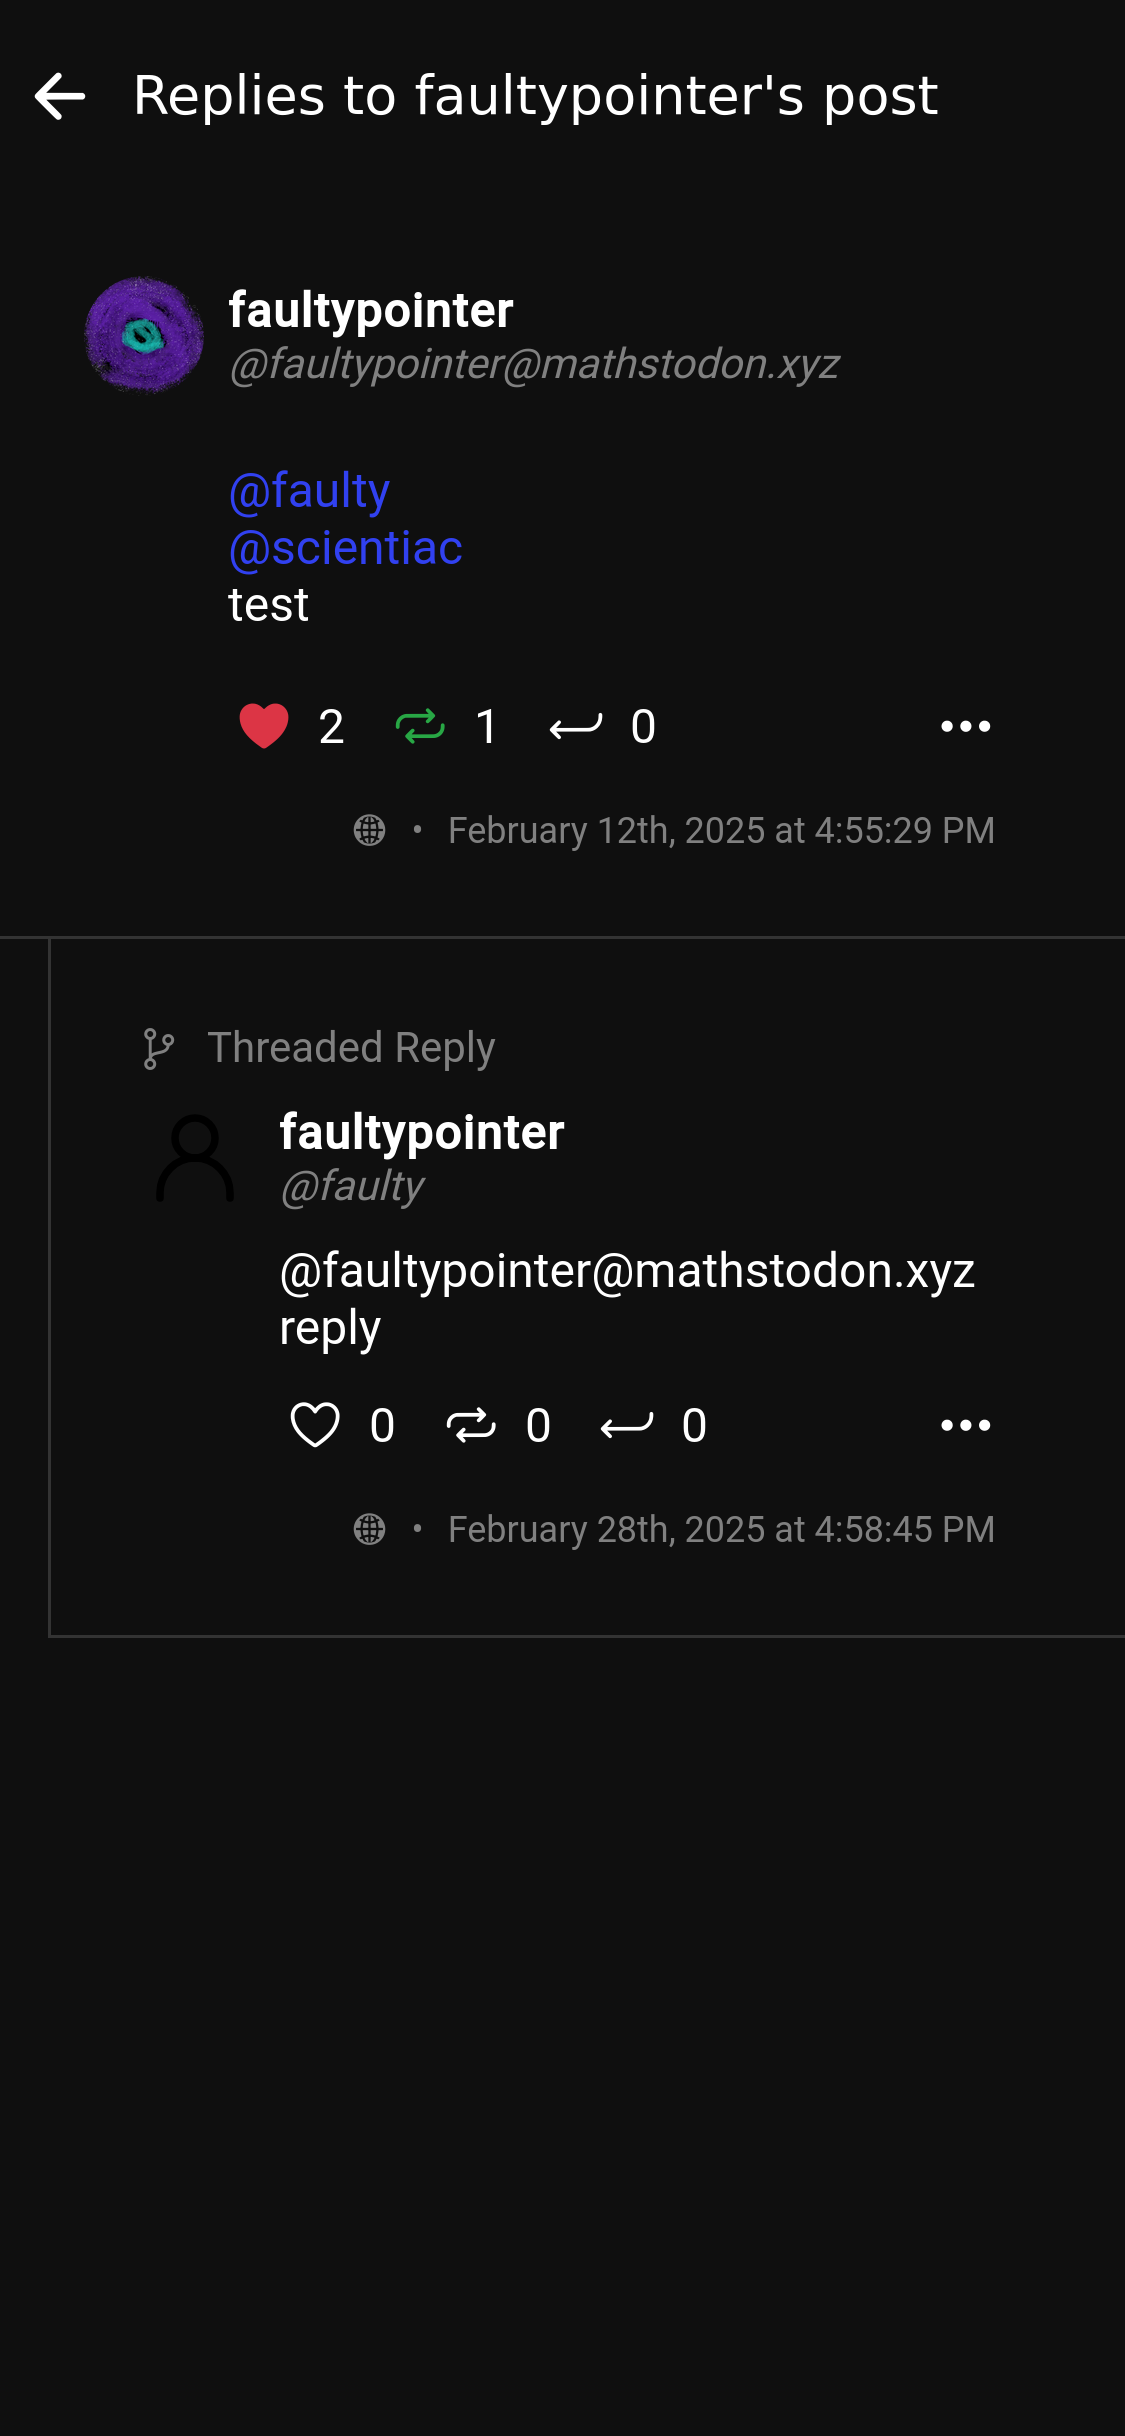
\includegraphics[width=\linewidth]{Graphics/replylikereboost.png}
    \caption{Liking, reboosting and replying to a post}
    \label{fig:like_reboost_reply}
  \end{minipage}
  \hfill % adds some space between images
  % Second image in its own minipage
  \begin{minipage}[b]{0.45\linewidth}
    \centering
    
\includegraphics[width=\linewidth]{Graphics/postreplies.png}
    \caption{Viewing all the replies to a post}
    \label{fig:post_replies}
  \end{minipage}
\end{figure}

\section{More: Notifications, Followers and Following}
Users can keep track of their interactions through notifications, as shown in Figure~\ref{fig:notifications}, which provides updates on likes, replies, and follows.

Additionally, users can manage their connections through the Following and Followers list (Figure~\ref{fig:following_list}), where they can see the accounts they are following and those who follow them.

\begin{figure}[htbp]
  \centering
  % First image in its own minipage
  \begin{minipage}[b]{0.45\linewidth}
    \centering
    \includegraphics[width=\linewidth]{Graphics/Notifications.png}
    \caption{Notifications of an account}
    \label{fig:notifications}
  \end{minipage}
  \hfill % adds some space between images
  % Second image in its own minipage
  \begin{minipage}[b]{0.45\linewidth}
    \centering
    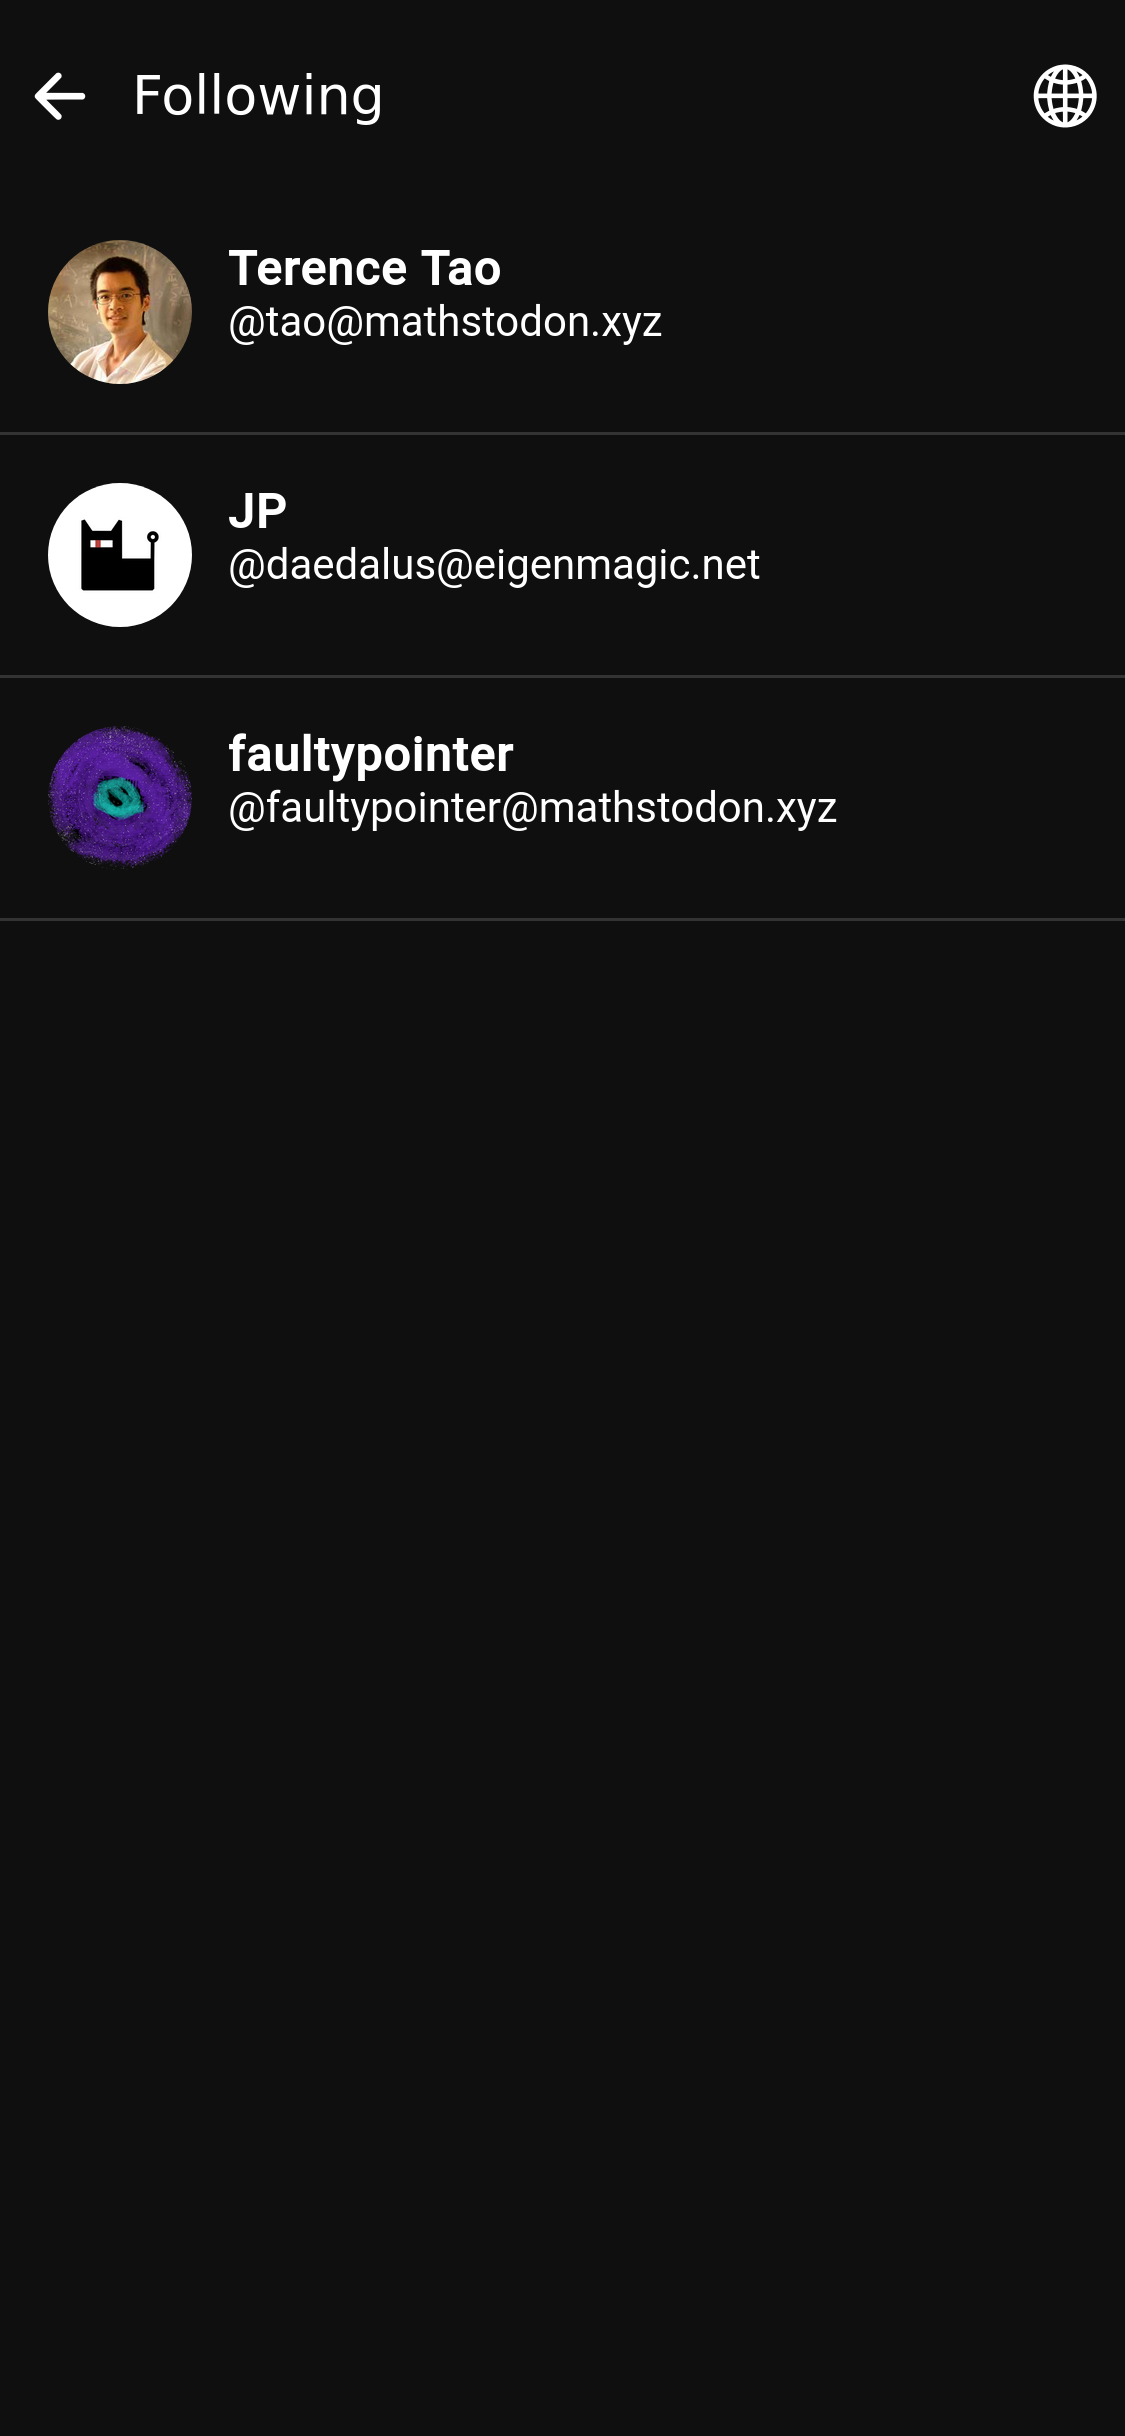
\includegraphics[width=\linewidth]{Graphics/followerandfollowing.png}
    \caption{Following list}
    \label{fig:following_list}
  \end{minipage}
\end{figure}


\chapter{CONCLUSION}

Here we write about what metohods we used to make the project possible.

\addcontentsline{toc}{chapter}{REFERENCES}
\renewcommand{\bibname}{\centering REFERENCES}
\bibliographystyle{IEEEtran}
\bibliography{references}

\addcontentsline{toc}{chapter}{APPENDIX}

\centering{\textbf{APPENDIX A}}
\vspace{1cm}

\newpage
\centering{\textbf{APPENDIX B}}
\vspace{1cm}





\end{document}
